\vspace{-0.4cm}
\section{Introduction}

Navigation systems have changed the way we drive and in particular affected how we plan our trips. Nowadays, they are not only used to find the shortest route in an unknown area but also to react to current events such traffic jams and accidents and compute the fastest route. The latter became possible due to the availability of real-time traffic data gathered from road sensors, GPS transmissions from vehicles and reporting tools for accidents. The most recent navigation systems (e.g., \cite{Pan13}) even go one step further and use the collected historic data to build traffic models in order to predict the future traffic. In conjunction with the real-time information, the ultimate goal is to provide a faster route and better estimation of the expected travel time to the user. Since a prediction model is involved in these systems, a main observation to be made is that the outcome, i.e., the estimated time for a route and thus the fastest route, can never be trusted with certainty and is subject to variation. Consequently, the fastest route is not necessarily the most reliable route, i.e., the route with the least variation in possible travel times. Reliability of a route is particularly important to users when a deadline, such as a flight departure or an important meeting, has to be met. 

To illustrate, consider the example in \cref{fig:motivation1}, where estimated total travel times for two routes with the same source and destination are given. Based on the \textit{expected} travel times, route A is the better choice. However, this result ignores the uncertain nature of traffic prediction. On the other hand, in \cref{fig:motivation2}, travel times for same two routes are given with some level of uncertainty, i.e., the travel times are given by a probability density function (\textit{pdf}). Continuing with our example in \cref{fig:motivation}, let us assume that the user has only 60 minutes to reach the destination in order to be on time. The probability that the user is at the destination in at most 60 minutes, is the sum of probabilities of travel times smaller or equal to 60 minutes. In the example in \cref{fig:motivation2}, the user has a chance of 99.2\% to reach his destination on time when choosing route B, whereas choosing route A gives him only an 89\% chance to be on time. Furthermore, if the user wants to achieve the same level of confidence using route A, he has to start 10 minutes earlier.

% \begin{figure}[h]
%     \centering
%     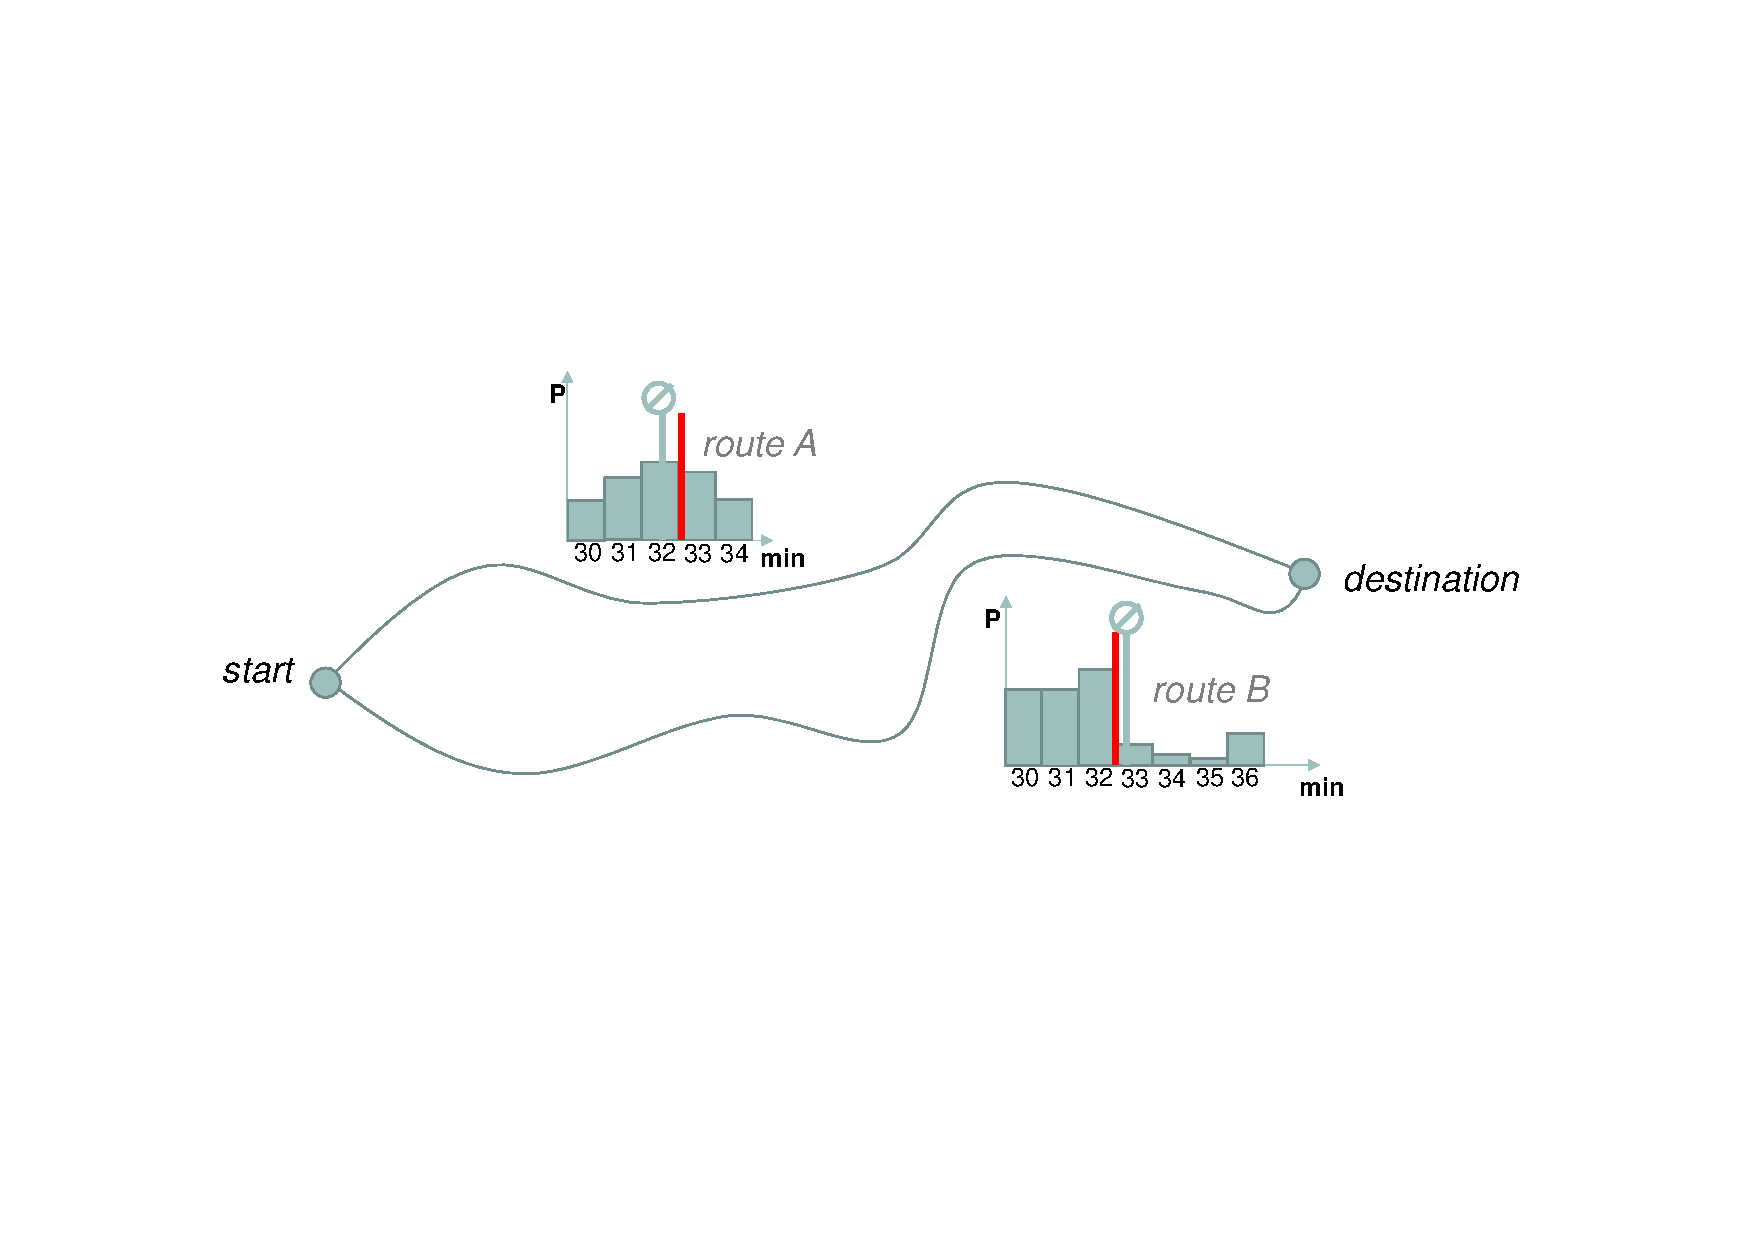
\includegraphics[width=0.90\columnwidth]{figures/motivation.pdf}
%     \caption{Probabilistic cost of two routes}
%     \label{fig:motivation}
% \end{figure}

\begin{figure}[t]
    \centering
    \subfigure[Deterministic result]{
        \label{fig:motivation1}
        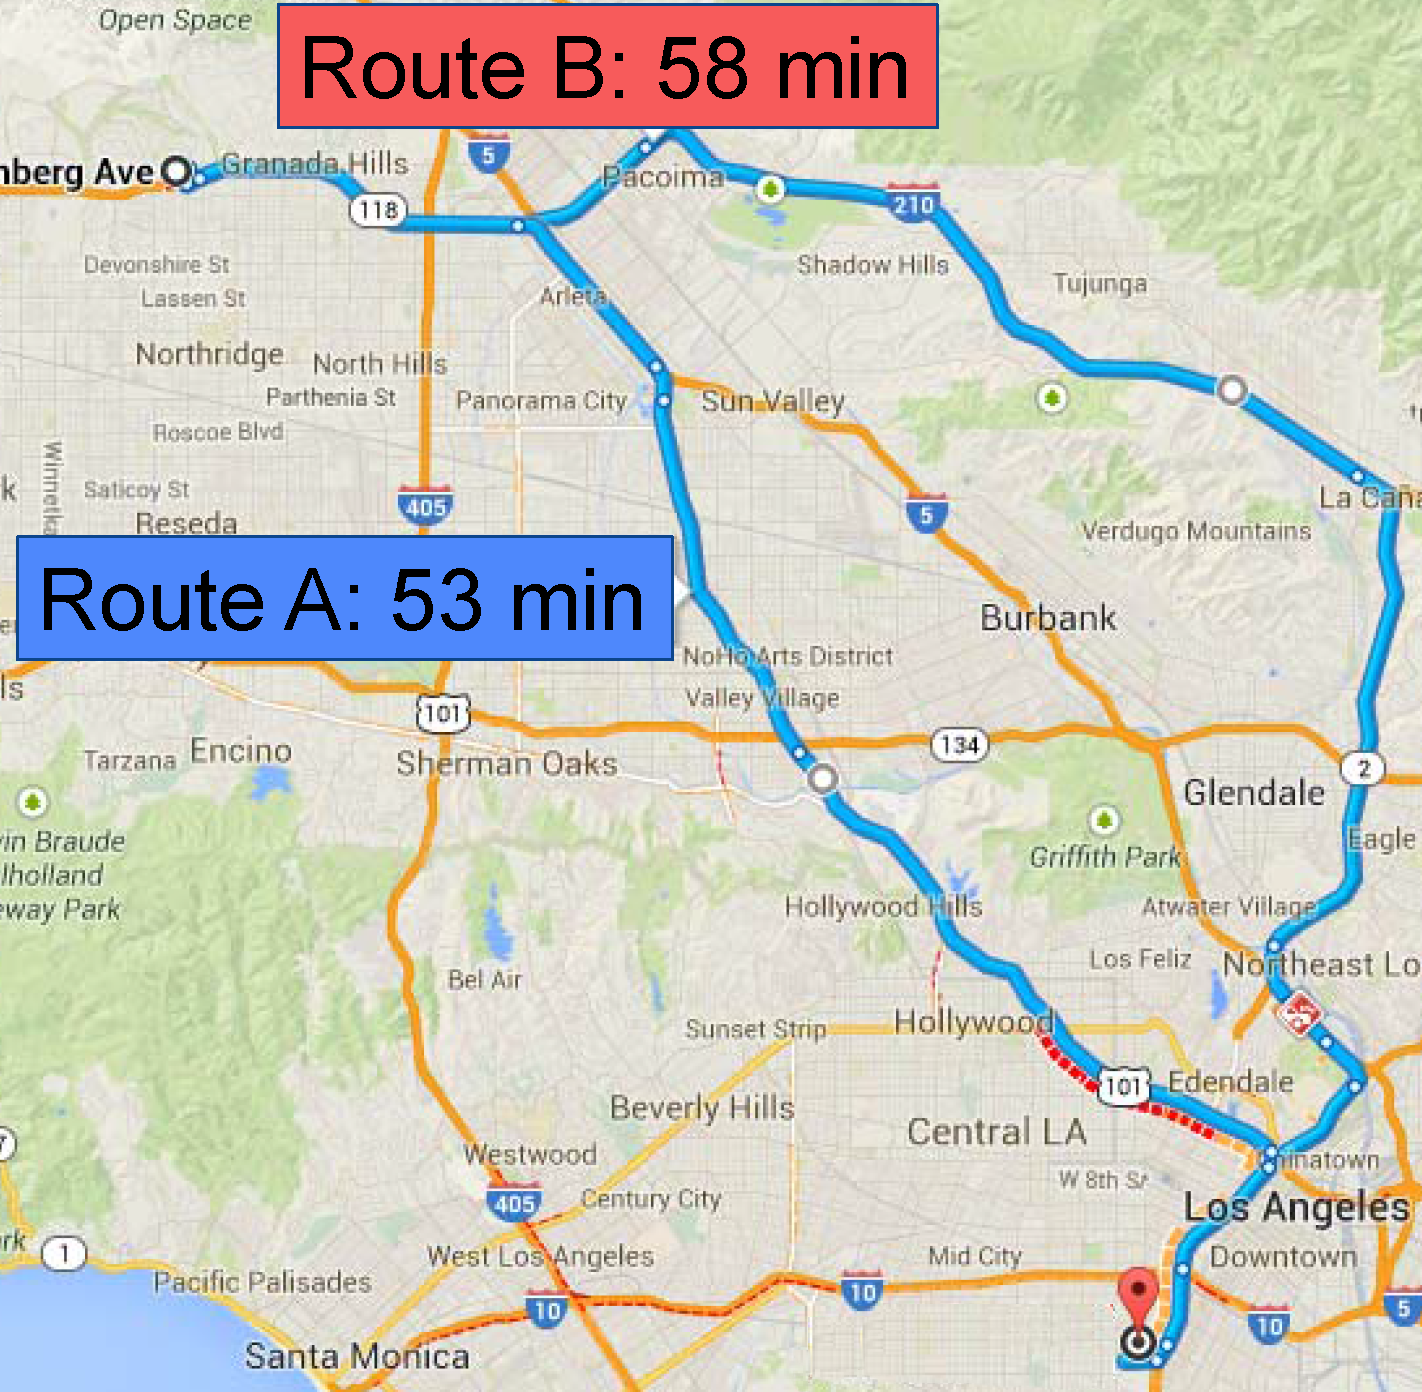
\includegraphics[width =
        0.38\columnwidth]{figures/motivation1_anonym.png} }
    \subfigure[Probabilistic result]{
        \label{fig:motivation2}
        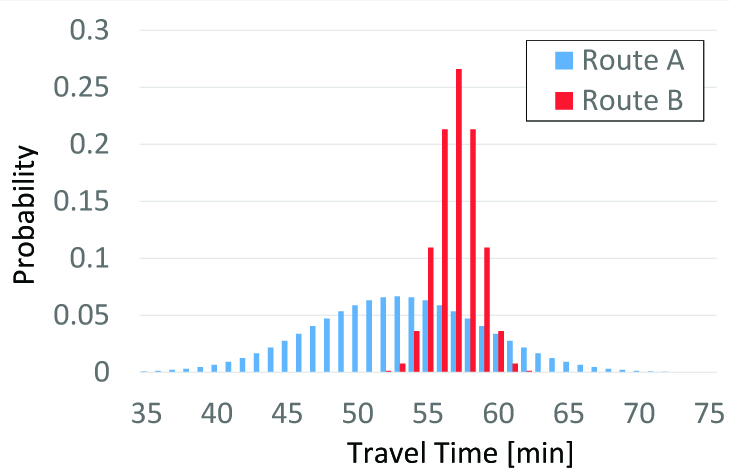
\includegraphics[width = 0.53\columnwidth]{figures/motivation2.jpg}
    }
    \vspace{-0.2cm}
    \caption{Estimated Travel Time of two paths}\label{fig:motivation}
    \vspace{-0.5cm}
\end{figure}

The example in \cref{fig:motivation} shows that similar to other applications \cite{Sarma08}, explicitly handling the uncertainty is better than ignoring it. Correspondingly, we believe that taking the uncertainty of the travel time into account will enable next-generation route planning applications by extending path queries to probabilistic path queries, allowing for queries such as:  \textit{What are the paths from my hotel to the airport whose travel times are at most 40 minutes with a probability of at least 95\%?}. 

To achieve this goal, we have to compute a \textit{pdf} for the travel times over a given route which gives the probability of each \textit{possible} travel time, being the \textit{actual} travel time of the route. Many solutions have been proposed to compute such \textit{pdf}. A common assumption in all these approaches is that the probabilistic link travel times (\textit{pltts}), i.e., the probabilistic times to travel each link on the route, is given a priori. In other words, these studies focus on computing a \textit{pdf} for the entire route by combining the \textit{pdfs} of all links in different ways. On the other hand, to the best of our knowledge, no study has focused on finding the \textit{pltt} for a single link. All existing techniques on predicting link travel times only provide a single estimated value for each link \cite{Pan13, Xu15} which is not compatible with the algorithms developed to compute the \textit{pdf} of a route. In this paper, we aim to fill in this gap by providing several techniques to compute \textit{pltts} in a road network.

Even though it is possible to evaluate these techniques by comparing how accurate they predict link travel times, the overall goal is yet to build a \textit{pdf} that predicts the travel time over a route as accurate as possible. For this reason, we utilize our \textit{pltt} computation techniques in different algorithms proposed for computing route \textit{pdfs}. In order to cover all different algorithms, we first classify them based on three basic characteristics; representation, time-dependency and correlation. The significance of the \textit{pltt} computation step becomes clear once we show that the accuracy of the \textit{pltts} directly impact the accuracy of the \textit{pdf} for the entire route. In fact, through experiments on real-world data, we show that utilizing a good algorithm for generating route \textit{pdfs} with a bad \textit{pltt} estimation technique, will result in a less accurate outcome compared to when a bad algorithm is utilized with a good \textit{pltt} estimation technique.\\
As mentioned earlier, no existing study has focused on \textit{pltt} computation. Consequently, no study has been able to perform an end to end evaluation of different algorithms for computing route \textit{pdfs}. For the first time, in this paper, we use real-world data sets to evaluate these algorithms. Evaluating the accuracy of a probabilistic prediction is a daunting task itself. We show how several existing methods such as expected distance, goodness-of-fit and scoring functions are incapable of this task. Therefore, we propose a solution which is capable of evaluating the accuracy of both \textit{pltts} and route \textit{pdfs}.\\
In sum, the contributions of this paper are as follows:
\begin{itemize}
\item Propose techniques to compute \textit{pltts} as a missing step towards computing a \textit{pdf} for travel times of a route (\cref{sec:lttestimation}).
\item Classify existing algorithms for computing route \textit{pdfs} based on their basic characteristics (\cref{sec:methods}).
\item Propose a measure capable of evaluating the accuracy of a probabilistic prediction (\cref{sec:evaluate}).
\item Conduct various experiments using real-world data to (1) compare different \textit{pltt} computation techniques, (2) perform an end-to-end comparison of different algorithms for building route \textit{pdfs} and more importantly (3) show the impact of \textit{pltt} computation in the overall process of generating route \textit{pdfs} (\cref{sec:experiments}).
\end{itemize} 

%With this goal in mind, in this work, we consider the problem of computing the \textit{pdf} of the travel time for one given path. This \textit{pdf} associates each possible travel time with the corresponding probability that the vehicle will need this time for completing the route. Specifically, we will make the following contributions:

%\begin{enumerate}
%\item \label{item:1} It turns out that all existing approaches considering uncertainty in traffic networks make the simplifying assumption that the probabilistic link travel times (\textit{pltts}), i.e., the predicted time for each road segment, are given. However, existing techniques on predicting link travel times provide a single value estimation only or are not compatible with existing techniques for computing the probabilistic link travel time of a path. Thus, there is a huge lack in taking the uncertainty of predictions into account and estimating not only accurate \textit{pltt} estimations but also possible correlations between them. We will fill this gap by providing techniques that yield \textit{pltts} by taking historic as well as real-time information into account.
%\item \label{item:2} Subsequently we focus on approaches for computing the probabilistic path travel times based on \textit{pltts}. After reviewing and categorizing the existing studies considering uncertainty in networks, we identify three basic characteristics (representation, time-dependency and correlation) and extract or adapt methods for all possible combinations of these characteristics for the ultimate goal of a fair and insightful comparison.
%\item The evaluation  of a probabilistic prediction is a daunting task. Neither expected distance measures nor goodness-of-fit methods nor primitive scoring functions are applicable. So far no evaluation of the accuracy for the methods in item \ref{item:2} has been performed. We propose adequate solutions to the evaluation problem and compare the accuracy of both the techniques in items \ref{item:1} and \ref{item:2} on a large real-world data set. Our results provide deep insights on the effect and functionality of all sub-modules.
%\end{enumerate}

%For the ultimate goal of providing this pipeline we avail ourselves of techniques from database, transportation, weather prediction and statistics research. One main question that this study will thus address is the usefulness and validity of the consideration of uncertainty for route planning applications.
% 
% \begin{itemize}
%   \item We review and categorize existing work for shortest path algorithms on
%   uncertain traffic networks with a particular focus on the computation of the
%   uncertain travel time of one path.
%   \item We consider the problem of the parameter generation. This involves
%   estimating uncertain link travel times and correlations between these.
%   \item 
%   \item All experiments are carried out on a large scale real-world dataset
% \end{itemize}

% The remainder of this paper is structured as follows: In Section
% \ref{sec:problemdef} we formally define the problem setting and crucial notations. We review
% important related work in Section \ref{sec:related}. In Section
% \ref{sec:lttestimation} we propose methods for the probabilistic prediction of
% edge weights and correlations. How these predictions can be used in order to
% compute a prediction for a whole path is discussed in Section \ref{sec:methods}.
% We then discuss measurements for evaluating probabilistic predictions in Section
% \ref{sec:evaluate}. In a broad experimental setting we show both the validity of
% the proposed estimation methods for the link travel times and a comparison of
% the approaches in terms of efficiency and accuracy in Section
% \ref{sec:experiments}. Section \ref{sec:conclusion} concludes the paper.

% Figure \ref{fig:component} illustrates the components of this work.
% \begin{figure}[h]
%     \centering
%     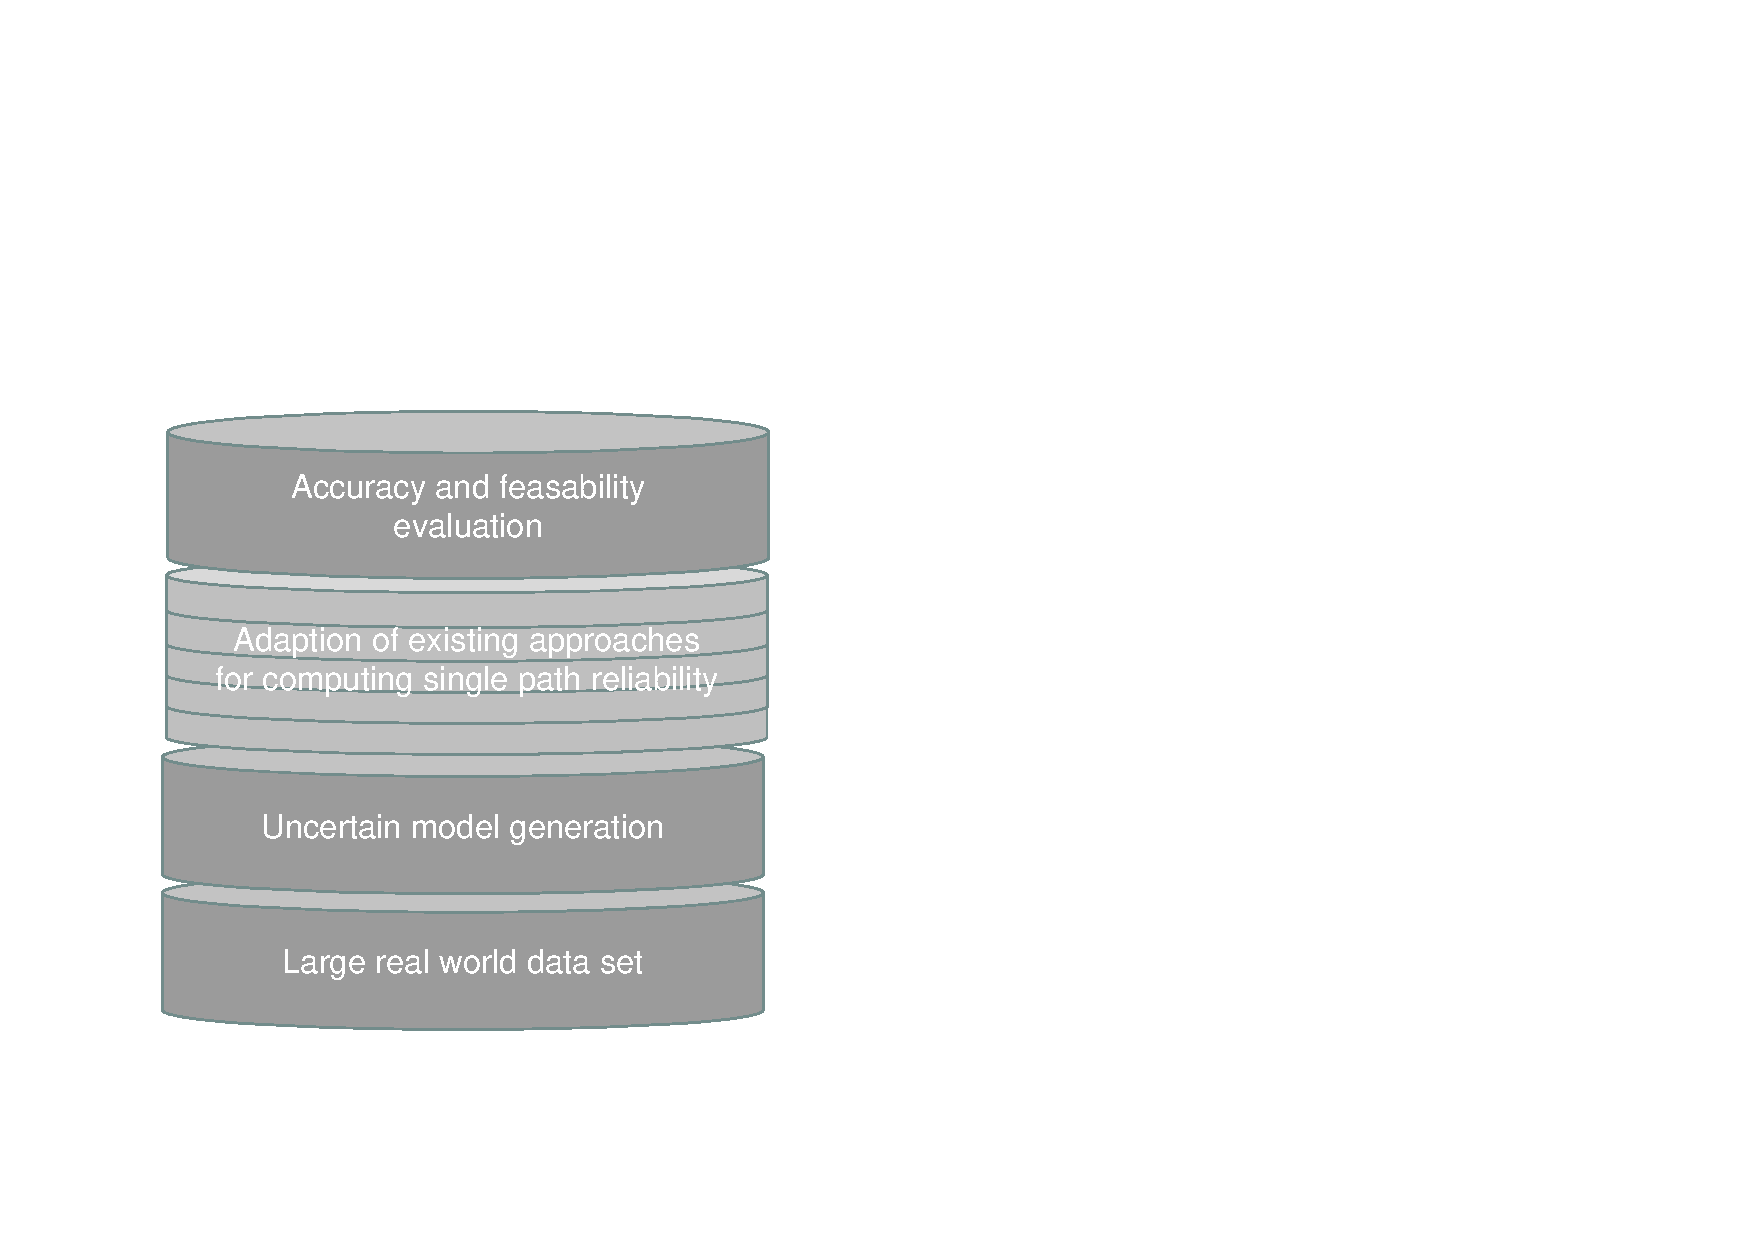
\includegraphics[width=0.50\columnwidth]{figures/contributions.pdf}
%     \caption{Components of this work}
%     \label{fig:component}
% \end{figure}


% ------Copy from \cite{NieWu09}-----------
% Another common definition of optimality in stochastic routing has to do with reliability, recognizing that a LET route (or
% policy) may be subject to high risks and therefore is not desirable to a
% risk averse
% traveler. For example, people tend to budget
% a large amount of time for travel when they plan for important events (e.g. job interviews). The key objective of routing in
% such a circumstance is to reduce the risk of arriving late rather than to minimize the expected travel time. In practice, how-
% ever, such risk averse behavior leads to excessively conservative time budgets. It is therefore necessary to both guarantee
% reliable on-time arrival and avoid unnecessary waiting. This paper precisely addresses the above problem.
% ------Copy end -----------